\documentclass[11pt,a4paper]{article}

\usepackage[T1]{fontenc}
\usepackage[utf8]{inputenc}
\usepackage{mathpazo}
\usepackage[margin=1in]{geometry}
\usepackage{microtype}
\usepackage{amsmath}
\usepackage{booktabs}
\usepackage{array}
\usepackage{xcolor}
\usepackage{listings}
\usepackage{enumitem}
\usepackage{tikz}
\usetikzlibrary{positioning,arrows.meta,calc}
\usepackage[colorlinks=true,linkcolor=accent,urlcolor=accent]{hyperref}

\definecolor{accent}{HTML}{1F4E79}
\definecolor{codebg}{HTML}{F6F8FA}
\definecolor{codeframe}{HTML}{D6DBE1}
\definecolor{kw}{HTML}{A3254A}
\definecolor{cmt}{HTML}{5A7D5A}
\definecolor{newbox}{HTML}{E8F0F8}

\lstdefinestyle{sqlstyle}{
  language=SQL,
  morekeywords={ASOF,LATERAL,EXPLAIN,COSTS,OFF,LIMIT},
  basicstyle=\ttfamily\small,
  keywordstyle=\color{kw}\bfseries,
  commentstyle=\color{cmt}\itshape,
  backgroundcolor=\color{codebg},
  frame=single, rulecolor=\color{codeframe},
  framesep=4pt, xleftmargin=4pt,
  breaklines=true, showstringspaces=false,
  columns=fullflexible, keepspaces=true,
}
\lstdefinestyle{plain}{
  basicstyle=\ttfamily\small,
  backgroundcolor=\color{codebg},
  frame=single, rulecolor=\color{codeframe},
  framesep=4pt, xleftmargin=4pt,
  columns=fullflexible, keepspaces=true,
}
\lstset{style=sqlstyle}

\setlist{itemsep=2pt,topsep=4pt}
\setlength{\parskip}{4pt}

\newcommand{\code}[1]{\texttt{#1}}
% file and function names, written as-is (underscores need no escaping)
\DeclareUrlCommand\src{\urlstyle{tt}\def\UrlBreaks{\do\/}}
% one file (or group of files) and what changed in it
\newcommand{\fileitem}[1]{\par\medskip\noindent{\color{accent}#1}\par\nopagebreak\noindent\ignorespaces}

\title{\textbf{ASOF JOIN for PostgreSQL}\\[4pt]
  \large CS631 Course Project Report}
\author{Deepjyoti Kakoti (26M0774) \and Debasish Bordoloi (26M0776) \and
  Shubh Karman Singh (26M0843)}
\date{November 2026\\[8pt]
  \normalsize Code and git history: \url{https://github.com/qascade/ASOF-Joins}}

\begin{document}
\maketitle

\begin{abstract}
An \emph{ASOF join} matches each row of one table with at most one row of another
table: the row whose time is closest to it, looking either backwards or forwards in
time, as the join condition says. For example, it matches each trade with the latest quote
that was valid when the trade happened. Many analytical databases support it, such as
DuckDB, ClickHouse, Snowflake, kdb+ and QuestDB, but PostgreSQL does not. We added
\code{ASOF JOIN} to PostgreSQL~18 in two phases. In the first phase the new syntax is
rewritten into an equivalent lateral join query that PostgreSQL can already run. In the
second phase ASOF becomes a real join type: the optimizer plans it as a sort followed by
a single merge pass, and a new executor operator runs it.
\end{abstract}

\tableofcontents
\bigskip

%=====================================================================
\section{The problem}
%=====================================================================

\subsection{What an ASOF join is}

Suppose a stock exchange records two tables. \code{trades} holds every trade, with its
symbol and time. \code{quotes} holds every price quote, also with symbol and time. To know
the price that was quoted when a trade happened, we need, for each trade, \emph{the latest
quote for the same symbol at or before the trade's time}.

\begin{center}
\begin{tabular}{@{}lll@{\hspace{3em}}lll@{}}
\toprule
\multicolumn{3}{c}{\code{trades}} & \multicolumn{3}{c}{\code{quotes}}\\
\cmidrule(r){1-3}\cmidrule(l){4-6}
sym & ts & qty & sym & ts & price \\
\midrule
A & 5 & 100 & A & 2 & 10\\
A & 9 & 50  & A & 4 & 11\\
B & 3 & 70  & A & 7 & 12\\
  &   &     & B & 6 & 20\\
\bottomrule
\end{tabular}
\end{center}

\noindent The answer is: trade \code{(A,5)} gets quote \code{(A,4)}, trade \code{(A,9)}
gets quote \code{(A,7)}, and trade \code{(B,3)} gets nothing, because the only B quote
comes later.

An ordinary join cannot express this. The join
$\texttt{t.sym = q.sym AND t.ts >= q.ts}$ returns \emph{every} earlier quote: two rows for
trade \code{(A,5)} and three for \code{(A,9)}. The ASOF join keeps only the nearest one.
A filter cannot do this, because a filter looks at one joined row at a time, while
choosing the nearest quote needs all the candidate quotes of a trade to be compared.

\subsection{How people write it in PostgreSQL today}
\label{sec:lateral}

Without ASOF support, users write a \emph{LATERAL} subquery, which runs once for each
trade:

\begin{lstlisting}
SELECT t.*, q.price
FROM trades t
LEFT JOIN LATERAL (
    SELECT q.price FROM quotes q
    WHERE q.sym = t.sym AND q.ts <= t.ts
    ORDER BY q.ts DESC
    LIMIT 1) q ON true;
\end{lstlisting}

This query is slow when there is no index on \code{quotes(sym, ts)}. Without such an
index, the subquery scans the whole \code{quotes} table once for every trade, so the work
grows as $n \times m$ for $n$ trades and $m$ quotes. With the index, each trade needs one
index lookup instead.

\subsection{What we built}

With our change, the same query is written as:

\begin{lstlisting}
SELECT t.*, q.price
FROM trades t ASOF LEFT JOIN quotes q
  ON t.sym = q.sym AND t.ts >= q.ts;
\end{lstlisting}

%=====================================================================
\section{The syntax and its meaning}
%=====================================================================

\subsection{Accepted grammar}

\begin{itemize}
  \item \code{a ASOF JOIN b ON ...} and \code{a INNER ASOF JOIN b ON ...}: inner ASOF join.
  \item \code{a LEFT ASOF JOIN b ON ...} and \code{a ASOF LEFT JOIN b ON ...} (the
        DuckDB spelling): left ASOF join.
  \item \code{RIGHT} and \code{FULL} ASOF joins are rejected with the error ``only INNER
        and LEFT ASOF joins are supported''. They are not implemented for now.
\end{itemize}

\code{ASOF} is a new keyword. It can still be used as an output column label
(\code{SELECT 1 AS asof}) and as a quoted name (\code{"asof"}), but a table or column
called \code{asof} must now be written in quotes.

\subsection{The rules}

The \code{ON} clause is a list of conditions joined by \code{AND}. It must contain
\textbf{exactly one} ASOF comparison with \code{<}, \code{<=}, \code{>} or \code{>=} between a
left-side expression and a right-side expression. We call it the \emph{match condition}.
The other conditions are usually equalities such as \code{t.sym = q.sym}, which we call
the \emph{keys}.

\begin{itemize}
  \item \textbf{Nearest.} For each left row, among the right rows with equal keys that
        satisfy the match condition, the join picks the one \emph{closest} to the left
        row. For \code{t.ts >= q.ts} that is the largest \code{q.ts}; for
        \code{t.ts <= q.ts} it is the smallest.
  \item \textbf{Strict or not.} \code{>=} and \code{<=} allow an exact tie in time;
        \code{>} and \code{<} do not.
  \item \textbf{LEFT versus INNER.} A left ASOF join returns every left row exactly once;
        a row with no match gets NULLs in the right columns. An inner ASOF join drops
        left rows with no match.
  \item \textbf{NULLs.} A NULL key or a NULL time on either side never matches, just as
        with \code{=}.
  \item \textbf{Ties.} If two right rows have the same key and the same time, either one
        may be returned. This is the same in both phases.
  \item \textbf{ON versus WHERE.} A condition in \code{WHERE} is checked \emph{after} the
        nearest row has been chosen. For example, \code{WHERE q.price > 10} means ``find
        the latest quote, then keep the row only if that quote's price is above 10''. It
        does not mean ``find the latest quote whose price is above 10''.
\end{itemize}

%=====================================================================
\section{Overall approach}
%=====================================================================

PostgreSQL handles a query in a fixed sequence of stages (Figure~\ref{fig:pipeline}). The
\emph{parser} turns the SQL text into a tree. The \emph{analyzer} resolves table and
column names. The \emph{planner} (optimizer) chooses how to run the query, and the
\emph{executor} runs the chosen plan.

\begin{figure}[h]
\centering
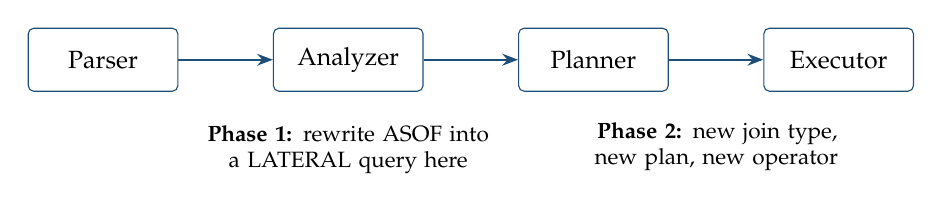
\begin{tikzpicture}[
  box/.style={draw=accent, rounded corners=2pt, minimum height=8mm,
              minimum width=19mm, font=\small, align=center},
  arr/.style={-{Stealth[length=2mm]}, thick, accent}]
  \node[box] (p) {Parser};
  \node[box, right=12mm of p] (a) {Analyzer};
  \node[box, right=12mm of a] (pl) {Planner};
  \node[box, right=12mm of pl] (e) {Executor};
  \draw[arr] (p) -- (a);
  \draw[arr] (a) -- (pl);
  \draw[arr] (pl) -- (e);
  \node[font=\footnotesize, below=3mm of a, align=center, text width=42mm]
    {\textbf{Phase 1:} rewrite ASOF into\\ a LATERAL query here};
  \node[font=\footnotesize, align=center, text width=48mm]
    at ($(pl.south)!0.5!(e.south) + (0,-7mm)$)
    {\textbf{Phase 2:} new join type,\\ new plan, new operator};
\end{tikzpicture}
\caption{Where each phase changes PostgreSQL.}
\label{fig:pipeline}
\end{figure}

We worked in two phases:

\begin{enumerate}
  \item \textbf{Phase 1: rewrite.} Parse the new syntax and immediately rewrite it into
        the LATERAL query shown above. Nothing after the analyzer changes. This gave us
        correct results quickly, and a reference to test against later.
  \item \textbf{Phase 2: native join.} Make ASOF a real join type that the planner
        understands, plan it as ``sort both the inputs, then merge them in one pass'', and
        write a new executor operator for it.
\end{enumerate}

Both versions stay in the code. A new setting chooses between them:

\begin{lstlisting}
SET enable_asofjoin_native = on;   -- default: the native join (Phase 2)
SET enable_asofjoin_native = off;  -- the LATERAL rewrite (Phase 1)
\end{lstlisting}

This lets us compare the results of the two, and gives users a fallback for
queries that the native join cannot run yet.

%=====================================================================
\section{Phase 1: the LATERAL rewrite}
%=====================================================================

\subsection{How it works}

The grammar was extended to accept the forms above and to mark the join as ASOF. At
the very start of the analyzer, before any names are resolved, the ASOF join is rewritten
into a lateral subquery:

\begin{itemize}
  \item the equality keys and the match condition move into the subquery's \code{WHERE};
  \item the subquery is sorted on the right side's time column, descending for \code{>}
        and \code{>=} and ascending for \code{<} and \code{<=}, so the nearest row comes
        first;
  \item \code{LIMIT 1} keeps only that row;
  \item a left ASOF join becomes \code{LEFT JOIN LATERAL ... ON true}, and an inner one
        becomes \code{JOIN LATERAL ... ON true}.
\end{itemize}

Because the rewrite happens so early, everything afterwards is unchanged PostgreSQL code.
The rewritten query and a hand-written LATERAL query produce the same plan.

\subsection{Limitations of the rewrite}

\begin{itemize}
  \item Since the rewrite runs before names are resolved, it has to recognise the two
        sides of the match condition by matching column names as text.
  \item The right-side operand of the match condition must be a plain column such as
        \code{q.ts}, not an expression such as \code{q.ts * 2}.
  \item The right side of the join must be a table or a named subquery.
  \item A view stores the rewritten query, so showing the view's definition prints a
        LATERAL subquery instead of \code{ASOF JOIN}.
  \item Most importantly, it is \emph{only as fast as the LATERAL query}: very slow
        without an index (Section~\ref{sec:lateral}).
\end{itemize}

%=====================================================================
\section{Phase 2: the native ASOF join}
%=====================================================================

\subsection{The idea: sort, then one merge pass}

If both the tables are sorted by \code{(sym, ts)}, the ASOF join can be done in one pass,
like a sort-merge join. We keep an iterator on the quotes table. For each trade, the
iterator moves forward over the quotes that have the same symbol and a time at or before
the trade's time. The last quote it passed is the answer for that trade. Because the
trades are also sorted, the next trade never needs a quote that is behind the iterator,
so the iterator will never move backwards.

After sorting, this costs $O(n + m)$, compared with $O(n \times m)$ for the LATERAL query
without an index. Sorting costs $O(n \log n + m \log m)$, and is skipped when an index
already provides the order.

\subsection{Analyzer changes}

When the switch is on, the analyzer no longer rewrites the query. Instead it:

\begin{itemize}
  \item gives the join one of two new join types, \code{ASOF\_INNER} or
        \code{ASOF\_LEFT};
  \item checks that the \code{ON} clause has exactly one usable match condition. A
        condition qualifies only if it uses one of \code{<}, \code{<=}, \code{>},
        \code{>=}, compares a left-side expression with a right-side expression, can be
        sorted, and has no random functions or subqueries in it. When no condition
        qualifies, the error names the reason (Section~\ref{sec:errors}).
\end{itemize}

The analyzer and the planner use the \emph{same} function to decide what counts as a match
condition, so they can never disagree.

\textbf{Hack.} Both new join types, \code{ASOF\_INNER} included, are added to
PostgreSQL's \src{IS_OUTER_JOIN} test. An inner ASOF join is not an outer join, but it
shares the property that matters: its \code{ON} conditions decide which rows match,
while \code{WHERE} conditions only filter the result, so the two must not be mixed.
Code that passes this test already keeps them apart: it picks sort keys only from the
\code{ON} conditions, estimates their selectivity separately, and puts them in a
different list in the plan (\code{Join Filter} versus \code{Filter}). ASOF joins get all
of this without our having to change each of those places one by one.

\subsection{Planner changes}

Most of the Phase 2 work is in the planner. The planner decides where each condition
should be checked, in what order to join the tables, and which join algorithm to use. An
ASOF join does not follow several of the planner's usual assumptions. The points below
describe each one and what we changed.

\paragraph{1. The match condition is not an ordinary condition.}
Normally the planner collects all conditions into one pool and lets any join algorithm
apply them as filters. If \code{t.ts >= q.ts} went into that pool, a hash join or nested
loop join would apply it as a filter and return \emph{every} earlier quote, which is
wrong. So the planner takes the match condition \emph{out} of the pool and stores it
privately with the ASOF join. Only the ASOF-specific code ever reads it.

\textbf{Hack.} The private place is a new field, \src{asof_clause}, added to
\src{SpecialJoinInfo}, the record the planner already keeps for each non-inner join.
The condition never enters the planner's normal lists of join conditions, so no other
part of the planner can see it, and none of them had to be changed to skip it.

The planner checks again that there is exactly one match condition, because simplifying
the query can change the \code{ON} clause after the analyzer has checked it.

Since the match condition is no longer in the pool, nothing would tell the table scans to
output the time columns. The planner therefore requests those columns explicitly.

\paragraph{2. The join order is fixed.}
For inner joins the planner may join tables in any order, and for outer joins it uses
well-known rules about which reorderings are safe. Those rules were not designed for ASOF
joins, and many of them do not hold. We treat an ASOF join like a \code{FULL} outer join,
which the planner never reorders. Other joins in the same query can still be reordered
around it.

\paragraph{3. Filters are not pushed below the join.}
The planner normally moves a filter such as \code{q.price > 10} down to the scan of
\code{quotes}, so that fewer rows reach the join. For an ASOF join this changes the
answer (it would find the latest quote \emph{with} price above 10). PostgreSQL already
refuses such a push-down for the right side of a left outer join, because that side may
be filled with NULLs. It does this by marking the right side's columns as ``possibly NULL
after this join''. We mark the right side of \emph{every} ASOF join this way, inner joins
included, so that filters stay above the join.

\textbf{Hack.} The marking is stored in each column reference's \src{varnullingrels}.
For an inner ASOF join it is not true: the right side is never filled with NULLs. We
set it anyway, because it is the existing mechanism that stops the planner from pushing
filters down, so no new mechanism was needed.

\paragraph{4. A left ASOF join can become an inner one.}
If a \code{WHERE} condition on the right side rejects NULLs (for example
\code{q.price > 10}), the NULL-filled rows of a left ASOF join would all be removed
anyway. The planner then treats it as an inner ASOF join, which is simpler to run. The
same rule already exists for ordinary left joins.

\paragraph{5. Only one join algorithm.}
For ordinary joins the planner compares nested loop, hash and merge join. For an ASOF
join it builds only the new \emph{ASOF join path}, because the other algorithms do not
know about the match condition.

\paragraph{6. Choosing the sort order.}
Both inputs are sorted first on the keys and then on the time column, for example
\code{(t.sym, t.ts)} and \code{(q.sym, q.ts)}. The sort direction of the time column
depends on the operator, so that one forward-only scan can handle all four operators:

\begin{center}
\begin{tabular}{@{}lll@{}}
\toprule
Match condition & Nearest means & Sort time column \\
\midrule
\code{t.ts >= q.ts}, \code{t.ts > q.ts} & largest earlier \code{q.ts} & ascending \\
\code{t.ts <= q.ts}, \code{t.ts < q.ts} & smallest later \code{q.ts} & descending \\
\bottomrule
\end{tabular}
\end{center}

In both cases, while scanning forward, the qualifying rows come first and the nearest one
is the \emph{last} qualifying row. So the executor does not need to know which operator
was used. It only checks whether the match condition is true for each row, and the
condition itself decides whether an exact tie counts. If the user wrote the condition the
other way round, for example \code{q.ts <= t.ts}, the planner flips it so the left
table's column is always on the left. NULLs are sorted last, since they never match.

\paragraph{7. Skipping unnecessary sorts.}
If an input is already in the needed order, for example because it is read through an
index on \code{(sym, ts)}, the planner skips its sort. To make this work, the planner had
to be told that the time column's order is useful; before this change it kept only the
order on \code{sym}.

\paragraph{8. Cost estimate.}
The planner compares plans by estimated cost. For the ASOF join path the cost is:
\[
  \text{cost} = \text{sort(left)} + \text{sort(right)}
   + c_{\text{cmp}} \cdot (n + m) + c_{\text{filter}} \cdot n
   + c_{\text{out}} \cdot \text{rows out},
\]
where each sort is counted only when it is needed. This is the same shape as the cost
of a sort-merge join.

\paragraph{9. Row count estimate.}
A left ASOF join returns exactly one row per left row, so the estimate is $n$ (reduced by
any \code{WHERE} filters). An inner ASOF join is estimated like a \emph{semijoin}: the
number of left rows that have at least one right row with an equal key.

\paragraph{10. Not supported in the planner.}
ASOF joins are not split across table partitions, and they are not run in parallel.

\subsection{The executor operator}
\label{sec:executor}

PostgreSQL's executor uses the \emph{iterator} model: each operator returns one row each
time its parent asks for the next one. The new \code{AsofJoin} operator reads its two
sorted inputs (Figure~\ref{fig:plan}).

\begin{figure}[h]
\centering
\begin{lstlisting}[style=plain]
Asof Join
  Merge Cond: (t.sym = q.sym)
  Asof Cond: (t.ts >= q.ts)
  Filter: (q.price > 10)
  ->  Sort
        Sort Key: t.sym, t.ts
        ->  Seq Scan on trades t
  ->  Sort
        Sort Key: q.sym, q.ts
        ->  Seq Scan on quotes q
\end{lstlisting}
\caption{The \code{EXPLAIN} output for \code{trades t ASOF LEFT JOIN quotes q ON t.sym =
q.sym AND t.ts >= q.ts WHERE q.price > 10}. The node says \code{Asof Join}, not
\code{Asof Left Join}, because the \code{WHERE} condition turned the left join into an
inner one (planner point~4).}
\label{fig:plan}
\end{figure}

\subsubsection{The algorithm}

The operator keeps an \emph{iterator} on the inner input (it points at the next unread
quote) and a \emph{best} row (the nearest quote found so far for the current key). For
each outer row (trade):

\begin{enumerate}
  \item If the trade's key is NULL, it has no match.
  \item If \emph{best} belongs to a different key than this trade, forget it.
  \item Move the iterator forward:
    \begin{itemize}
      \item while the quote's key is \emph{smaller} than the trade's key, skip it: no
            later trade can want it;
      \item while the quote has the \emph{same} key and satisfies the match condition,
            copy it into \emph{best} and move on;
      \item otherwise stop: the quote belongs to a later key or is too late in time.
    \end{itemize}
  \item Check \emph{best} against this trade once more. If it passes, output the trade
        with \emph{best}.
  \item If there is no match: in a left join output the trade with NULLs; in an inner
        join output nothing.
  \item Apply any \code{WHERE} filters to the output row.
\end{enumerate}

\subsubsection{Why it is correct}

Within one key, trades come in increasing time. Any quote that is early enough for one
trade is also early enough for every later trade with the same key. So the quotes the
iterator has passed never need to be seen again, and the last one passed is the nearest.
For \code{<} and \code{<=} the same argument holds with both the sides sorted descending.

The re-check in step~4 handles one special case: a trade with a NULL time. \emph{Best}
may still hold a quote from the previous trade, and the re-check makes sure that quote is
not returned.

\subsubsection{Keeping the best row}

The best row is \emph{copied} into memory owned by the operator. The input operator
reuses the same memory for every row it returns. If we kept only a pointer to the best
row, its values would change as soon as the iterator moved to the next quote.

\subsubsection{What the operator does not handle yet}
\label{sec:executor-limits}

The native operator currently needs \textbf{exactly one} equality key, and supports no
\code{ON} conditions other than the key and the match condition (conditions on the right
table alone are allowed, because they can be applied to the right table before the join).
Queries outside these limits fail with an error that names the limit and suggests turning
the switch off, so the LATERAL rewrite answers them.

The reason for the second limit: a condition such as \code{t.qty + q.price > 100} can
reject a quote for one trade but accept it for a later trade. A single forward pass has
already moved past that quote, so supporting such conditions needs a different design.

\subsection{Showing the join to users}

\begin{itemize}
  \item \code{EXPLAIN} prints \code{Asof Join} or \code{Asof Left Join}, with separate
        lines for the keys (\code{Merge Cond}), the match condition (\code{Asof Cond}),
        other \code{ON} conditions (\code{Join Filter}) and \code{WHERE} conditions
        (\code{Filter}), as in Figure~\ref{fig:plan}.
  \item \code{EXPLAIN ANALYZE} reports how many rows each filter removed.
  \item Views that use a native ASOF join print back as \code{ASOF JOIN} or
        \code{LEFT ASOF JOIN}, so \code{pg\_dump} and \code{\textbackslash d+} work.
\end{itemize}

%=====================================================================
\section{Code changes, file by file}
\label{sec:code}
\begin{sloppypar}
%=====================================================================

This section says \emph{where} each part of the work lives in the PostgreSQL source
code and \emph{what} was changed there. PostgreSQL's C code is in \src{src/backend}, and
its header files, which define the shared data structures, are in \src{src/include}.
Below, paths starting with \src{backend/} or \src{include/} are relative to \src{src/}.
In total the project changed or added 36 files under \src{src/}, about 2,100 lines,
not counting test files.

\begin{table}[h]
\centering
\small
\begin{tabular}{@{}p{3.1cm}>{\raggedright\arraybackslash}p{11.2cm}@{}}
\toprule
Stage & Main files \\
\midrule
Grammar & \src{include/parser/kwlist.h}, \src{backend/parser/gram.y},
          \src{include/nodes/primnodes.h} \\
Analyzer & \src{backend/parser/parse_clause.c}, \src{backend/optimizer/util/clauses.c} \\
Switch & \src{backend/utils/misc/guc_tables.c}, \src{backend/optimizer/path/costsize.c} \\
Preprocessing & \src{backend/optimizer/prep/prepjointree.c} \\
Conditions & \src{backend/optimizer/plan/initsplan.c} \\
Join search & \src{backend/optimizer/path/joinrels.c}, \src{joinpath.c},
              \src{pathkeys.c}, \src{costsize.c}, \src{backend/optimizer/util/pathnode.c} \\
Plan & \src{backend/optimizer/plan/createplan.c}, \src{setrefs.c}, \src{subselect.c} \\
Executor & \src{backend/executor/nodeAsofjoin.c} (new), \src{execProcnode.c} \\
Display & \src{backend/commands/explain.c}, \src{backend/utils/adt/ruleutils.c} \\
Data structures & \src{include/nodes/nodes.h}, \src{pathnodes.h}, \src{plannodes.h},
                  \src{execnodes.h} \\
\bottomrule
\end{tabular}
\caption{Where each stage of the work lives.}
\label{tab:files}
\end{table}

\subsection{New syntax (used by both phases)}

  \fileitem{\src{include/parser/kwlist.h}}
    One line adds \code{asof} to PostgreSQL's keyword list. Its category means it can
    still be used as a column label in \code{SELECT ... AS asof}.

  \fileitem{\src{backend/parser/gram.y}}
    This is the grammar, from which the parser is generated. We added the \code{ASOF}
    token, gave it the same precedence as \code{JOIN}, \code{LEFT} and the other join
    words so that the grammar has no ambiguities, and added three new rules to
    \src{joined_table}: \code{a ASOF JOIN b ON ...}, \code{a LEFT/INNER ASOF JOIN b ON
    ...} and \code{a ASOF LEFT/INNER JOIN b ON ...}. Each rule builds the usual join node
    (\src{JoinExpr}) and sets a new flag on it. The last two rules reject \code{RIGHT}
    and \code{FULL} with an error that points at the offending word.

  \fileitem{\src{include/nodes/primnodes.h}}
    The join node \src{JoinExpr} gets one new field, \code{bool isAsof}. PostgreSQL
    generates the code that copies, compares, saves and loads nodes from these header
    files, so the new field needs no hand-written support code.

\subsection{Phase 1: the rewrite}

  \fileitem{\src{backend/parser/parse_clause.c}}
    \src{transformFromClauseItem} is the function that analyses each item in the
    \code{FROM} clause. When it meets a join with \src{isAsof} set and the switch is
    off, it first calls the new function \src{transformAsofToLateralJoin}. That function
    builds, out of raw parse-tree nodes, exactly the SQL a user would have typed: a
    \code{SELECT *} over the right table, with the \code{ON} conditions as its
    \code{WHERE}, an \code{ORDER BY} on the right time column in the right direction,
    and \code{LIMIT 1}. It wraps this in a \emph{lateral} subquery that keeps the right
    table's name, so that \code{q.price} elsewhere in the query still works, and
    returns a new join whose \code{ON} is just \code{true}. It makes a new tree instead
    of changing the old one, because PostgreSQL may reuse a parse tree (for example for
    a prepared statement).

    Small helpers (\src{asofIsRightColumn}, \src{asofIsLeftOnly},
    \src{asofRefWalker}) decide which side an expression belongs to by looking at the
    table names written in it, since names are not resolved yet at this point.

  \fileitem{\src{test.sql}} (at the top of the repository)
    A self-checking script that runs each ASOF query next to a hand-written LATERAL
    query and prints \code{PASS} or \code{FAIL}.

\subsection{Phase 2: the switch and the new join types}

  \fileitem{\src{backend/utils/misc/guc_tables.c}, \src{backend/optimizer/path/costsize.c},
        \src{include/optimizer/cost.h}}
    PostgreSQL's settings are declared in a table in \src{guc_tables.c}. We added
    \src{enable_asofjoin_native} there (default \code{on}, changeable per session).
    The variable itself lives in \src{costsize.c} next to the other
    \src{enable_*} settings, and is also listed in
    \src{backend/utils/misc/postgresql.conf.sample}.

  \fileitem{\src{include/nodes/nodes.h}}
    The list of join types, \src{JoinType}, gets two new values, \src{JOIN_ASOF_LEFT}
    and \src{JOIN_ASOF_INNER}. Both are added to the \src{IS_OUTER_JOIN} test, so code
    that asks ``is this an outer join?'' treats ASOF joins with the same caution.

\subsection{Phase 2: analyzer}

  \fileitem{\src{backend/parser/parse_clause.c}}
    When the switch is on, \src{transformFromClauseItem} skips the rewrite. After the
    \code{ON} clause has been analysed, it changes the join type to
    \src{JOIN_ASOF_LEFT} or \src{JOIN_ASOF_INNER} and calls the new
    \src{checkAsofMatchClause}. That function looks at every condition in the
    \code{ON} clause, and if none is a usable match condition (or more than one is), it
    raises the error for the most specific reason, pointing at that condition. Later in
    the same function, \src{markRelsAsNulledBy} is called on the right side of every
    ASOF join. This is the marking that keeps \code{WHERE} filters above the join
    (planner point~3 above).

  \fileitem{\src{backend/optimizer/util/clauses.c}, \src{include/optimizer/optimizer.h}}
    \src{classify_asof_match_clause} examines one condition and returns either
    ``usable'' or the reason it is not: not a comparison, an equality (that is a key),
    one-sided, an operator such as \code{<>}, a type that cannot be sorted, a random
    function, a subquery, or a side that uses both tables. The reasons are an
    \src{enum} in \src{optimizer.h}, listed from least to most specific, which is how
    the analyzer chooses which error to show. \src{find_asof_match_clauses} returns the
    usable conditions. Both the analyzer and the planner call these two functions,
    which is why they always agree.

\subsection{Phase 2: planner}

  \fileitem{\src{backend/optimizer/prep/prepjointree.c}}
    Early clean-up steps that already had a case for each join type now have one for
    ASOF joins too, treated like left joins when subqueries are merged into the main
    query. In \src{reduce_outer_joins_pass2}, a left ASOF join becomes an inner ASOF
    join when a \code{WHERE} condition rejects NULLs from its right side (planner
    point~4).

  \fileitem{\src{backend/optimizer/plan/initsplan.c}}
    This file decides where every condition is checked. In
    \src{deconstruct_distribute} we find the match condition again, remove it from the
    join's list of conditions, and store it in the new field
    \src{SpecialJoinInfo.asof_clause} (planner point~1). We also register both of its
    sides as sortable expressions, which is what later lets an index on
    \code{(sym, ts)} report that its order is useful, and ask the table scans to output
    the time columns (\src{add_vars_to_targetlist}). In \src{make_outerjoininfo}, ASOF
    joins get the same fixed-order treatment as \code{FULL} joins (planner point~2).
    \src{rebuild_joinclause_attr_needed} re-adds the time columns when the planner
    recomputes which columns are needed.

  \fileitem{\src{include/nodes/pathnodes.h}}
    Adds the field \src{asof_clause} to \src{SpecialJoinInfo}, the record the planner
    keeps for each non-inner join, and the new structure \src{AsofJoinPath}, which
    describes one candidate way to run the join: its two inputs, the key conditions,
    the match condition, the two flags (descending, strict) and the sort order for each
    input.

  \fileitem{\src{backend/optimizer/path/joinrels.c}}
    In \src{populate_joinrel_with_paths}, the rules for when the join result is
    certainly empty: an inner ASOF join is empty if either input is, a left ASOF join
    only if its left input is. In \src{try_partitionwise_join}, ASOF joins return
    early, so they are never split across partitions.

  \fileitem{\src{backend/optimizer/path/joinpath.c}}
    \src{add_paths_to_joinrel} is where the planner normally tries nested loop, merge
    and hash join. At its top, ASOF joins are sent to the new \src{add_asofjoin_path}
    and the function returns, so no other algorithm is tried (planner point~5).
    \src{add_asofjoin_path}:
    \begin{itemize}
      \item reuses the merge-join helpers to pick the key columns and their order;
      \item flips the match condition if the right table was written first, and picks
            the sort direction and the strict flag from the operator (planner point~6),
            using \src{asof_match_opfamilies} to find how the operator's types are
            sorted;
      \item appends the time column to each side's sort order
            (\src{append_asof_pathkey}, which skips it when it would be redundant);
      \item tries both the cheapest way to read each input (which then needs a Sort)
            and the cheapest way that is already in the right order, such as an index
            scan (no Sort), and lets the planner keep the cheapest combination
            (planner point~7).
    \end{itemize}

  \fileitem{\src{backend/optimizer/path/pathkeys.c}}
    The planner throws away a sort order that it thinks no later step will use. Before
    our change it kept an index's order on \code{sym} but cut off \code{ts}. The new
    \src{is_asof_match_eclass} recognises the ASOF time column, and
    \src{pathkeys_useful_for_merging} now keeps that part of the order in either
    direction.

  \fileitem{\src{backend/optimizer/util/pathnode.c}, \src{include/optimizer/pathnode.h}}
    \src{create_asofjoin_path} fills in an \src{AsofJoinPath}, marks it as not to be
    run in parallel, and calls the cost function.

  \fileitem{\src{backend/optimizer/path/costsize.c}}
    \src{cost_asofjoin} computes the cost formula of planner point~8.
    \src{calc_joinrel_size_estimate} gets the two row estimates of planner point~9.
    In \src{backend/utils/adt/selfuncs.c} and \src{network_selfuncs.c}, the functions
    that estimate how selective an equality is treat ASOF joins like semijoins.

  \fileitem{\src{backend/optimizer/plan/createplan.c}, \src{include/nodes/plannodes.h}}
    Once the cheapest path is chosen, \src{create_asofjoin_plan} turns it into an
    \src{AsofJoin} plan node, the structure the executor reads. It adds a Sort node
    under each input that needs one, writes every condition with the left table's
    expression on the left, puts \code{ON} conditions and \code{WHERE} conditions in
    separate lists (\code{Join Filter} and \code{Filter}), and records for each key the
    exact comparison rules the Sort used (function, collation, direction, NULL
    position).

  \fileitem{\src{backend/optimizer/plan/setrefs.c}, \src{subselect.c}}
    Final touches done for every plan node: \src{set_join_references} rewrites each
    column reference in the key and match conditions as ``column $k$ of the left
    input'' or ``column $k$ of the right input'', which is how the executor finds
    values; \src{finalize_plan} records which query parameters the conditions use.

\subsection{Phase 2: executor}

  \fileitem{\src{backend/executor/nodeAsofjoin.c}} (new file, about 375 lines)
    The new operator. Like every PostgreSQL operator it has three entry points:
    \begin{itemize}
      \item \src{ExecInitAsofJoin} runs once at start-up. It first calls
            \src{asof_check_supported}, which raises the ``not supported'' errors
            (unless the query is only being \code{EXPLAIN}ed). It then starts both
            inputs, compiles the conditions, prepares one comparison function per key
            with \src{asof_setup_keys} (the same recipe the existing merge join uses),
            and creates a private slot to hold the best row and an all-NULL row for
            unmatched outer rows.
      \item \src{ExecAsofJoin} returns the next output row. It is the algorithm of
            Section~\ref{sec:executor}, built from small helpers:
            \src{asof_compare_keys}, \src{asof_outer_key_is_null},
            \src{asof_cond_holds}, \src{asof_advance_inner} and \src{asof_clear_best}.
      \item \src{ExecEndAsofJoin} shuts the two inputs down.
    \end{itemize}

  \fileitem{\src{include/nodes/execnodes.h}}
    \src{AsofJoinState} holds what the operator remembers between calls: the compiled
    keys and their comparison functions, the compiled match condition, the inner
    cursor and an end-of-input flag, the best-row slot and a ``have best'' flag, and
    the all-NULL row.

  \fileitem{\src{include/executor/nodeAsofjoin.h}, \src{backend/executor/execProcnode.c},
        \src{Makefile}, \src{meson.build}}
    Declare the entry points, tell the executor's central dispatch functions to call
    them for an \src{AsofJoin} node, and add the new file to both build systems.

\subsection{Phase 2: showing the join}

  \fileitem{\src{backend/commands/explain.c}}
    Gives the node its name (\code{Asof Join}, \code{Asof Left Join}), prints the
    \code{Merge Cond}, \code{Asof Cond}, \code{Join Filter} and \code{Filter} lines, and
    under \code{EXPLAIN ANALYZE} the number of rows each filter removed.

  \fileitem{\src{backend/utils/adt/ruleutils.c}}
    \src{get_from_clause_item} turns a stored query back into SQL text. It now prints
    \code{ASOF JOIN} and \code{LEFT ASOF JOIN}, which is what makes view definitions
    and \code{pg\_dump} work.

\subsection{Bookkeeping}

  \fileitem{\src{include/catalog/catversion.h}}
    Views are stored on disk as query trees, and those trees can now contain the new
    join types. The catalog version number was raised so that a database created by an
    older build is not opened by this one by mistake.

  \fileitem{\src{backend/nodes/gen_node_support.pl}}
    This script generates node support code and normally checks that existing node
    numbers never change. Adding new node types shifts them, so that check was turned
    off for this development tree.

\end{sloppypar}

%=====================================================================
\section{Error messages}
\label{sec:errors}
%=====================================================================

A wrong \code{ON} clause gets an error that names the actual problem and points at the
condition responsible:

\begin{center}
\small
\begin{tabular}{@{}>{\ttfamily}p{5.2cm}p{9cm}@{}}
\toprule
\normalfont Example condition & Error \\
\midrule
t.sym = q.sym \textrm{(only)} & must contain an inequality (with a hint showing an example) \\
t.ts >= q.ts AND t.qty < q.price & must contain exactly one inequality \\
t.ts >= q.ts + t.qty & each side of the match condition must use only one input \\
t.ts <> q.ts & operator \code{<>} cannot be used as the match condition \\
q.ts >= 3 & must compare the left input with the right input \\
t.ts >= q.ts + random() & cannot contain volatile functions \\
t.ts >= (SELECT ...) & cannot contain a subquery \\
\bottomrule
\end{tabular}
\end{center}

When several conditions are wrong, the most specific reason is reported. Queries that are
valid but outside the native operator's limits get a separate error naming the limit (no
equality key, more than one, or an extra \code{ON} condition) and a hint to turn
\src{enable_asofjoin_native} off.

%=====================================================================
\section{Testing}
%=====================================================================

\subsection{Comparing the two phases}

The main correctness test is a \emph{differential} one. Each of 83 queries is run twice,
once with the switch off (the LATERAL rewrite, which is simple enough to use as the
reference) and once with it on (the native join). The two results are compared row by row in both directions. The test also
checks that the native plan really contains an ASOF join node, so a query that silently
fell back to another plan cannot pass.

The queries cover every operator with inner and left joins; integer, date, timestamp,
floating point (including NaN and infinity) and text columns; \code{WHERE} filters on
either side; subqueries, views and aggregates as inputs; other joins above and below the
ASOF join; two ASOF joins in a row; \code{ORDER BY ... LIMIT}; \code{WITH} queries;
prepared statements; inputs sorted by an index; and sorts large enough to spill to disk.

\textbf{Result: no wrong answers.} 74 of the 83 queries run on both paths, and each of them
returns identical rows on both. The other 9 stop with an error on one path: 4 are outside
the native operator's limits (Section~\ref{sec:executor-limits}), 2 are queries the
LATERAL rewrite cannot run, and 3 are valid queries that the native planner rejects (see
Section~\ref{sec:limits}).

%=====================================================================
\section{Limitations and future work}
\label{sec:limits}
%=====================================================================

\begin{itemize}
  \item \textbf{One equality key.} The native operator needs exactly one key. Zero keys
        or several keys should be a small extension, since the comparison code already
        works with lists of keys.
  \item \textbf{Extra ON conditions.} Conditions that use only the left table could be
        checked on the chosen pair cheaply. Conditions that use both tables need the
        operator to keep a whole key group and fall back to the next nearest row.
  \item \textbf{Simplified ON clauses.} Two valid queries are rejected by the native
        planner: an \code{ON} clause that simplifies to \code{false} (for example
        \code{... AND 1 = 0}), and a right-side subquery whose time column is a constant.
        Simplifying the query removes the match condition before the planner sees it.
        The LATERAL rewrite answers both correctly.
  \item \textbf{Restarting the operator.} The operator cannot yet be restarted, which is
        needed when it runs inside a correlated subquery.
  \item \textbf{Estimates.} The row estimate for an inner ASOF join ignores the match
        condition, so it is too high when many left rows come before all right rows.
  \item \textbf{Parallel and partitioned execution} are not supported.
  \item \textbf{RIGHT and FULL ASOF joins} are not supported.
\end{itemize}

%=====================================================================
\section{Conclusion}
%=====================================================================

We added \code{ASOF JOIN} to PostgreSQL~18 in two steps. The first step, a rewrite into a
LATERAL query, gave correct results with very little code and became the reference for
testing. The second step made ASOF a real join type with its own planning and its own
executor operator. The operator sorts both the inputs once and reads them together in
one pass, so it does not depend on an index the way the LATERAL query does.

In the second step, the match condition looks like an ordinary join condition, but the
planner must not treat it like one. Most of the planner work was therefore about keeping
the planner's usual steps away from it: taking it out of the shared pool of conditions,
keeping filters above the join, fixing the join order, and allowing only one join
algorithm. The sort direction of the time column is chosen from the operator, so one
forward-only scan handles all four comparison operators.

A setting keeps both versions available. A differential test of 83 queries finds no
query on which the two versions return different rows.

%=====================================================================
\section*{AI usage statement}
\addcontentsline{toc}{section}{AI usage statement}
%=====================================================================

We used an AI assistant (Claude, through Claude Code) during this project for the
following tasks:

\begin{itemize}
  \item understanding the structure of the PostgreSQL code and what its various
        functions do;
  \item finding the files that we needed to change for our use case;
  \item regression testing and creating test cases;
  \item managing our GitHub issues.
\end{itemize}

\end{document}
